\chapter{Theoretische Grundlage}
\begin{wrapfigure}[26]{R}[34pt]{0.6\textwidth}

  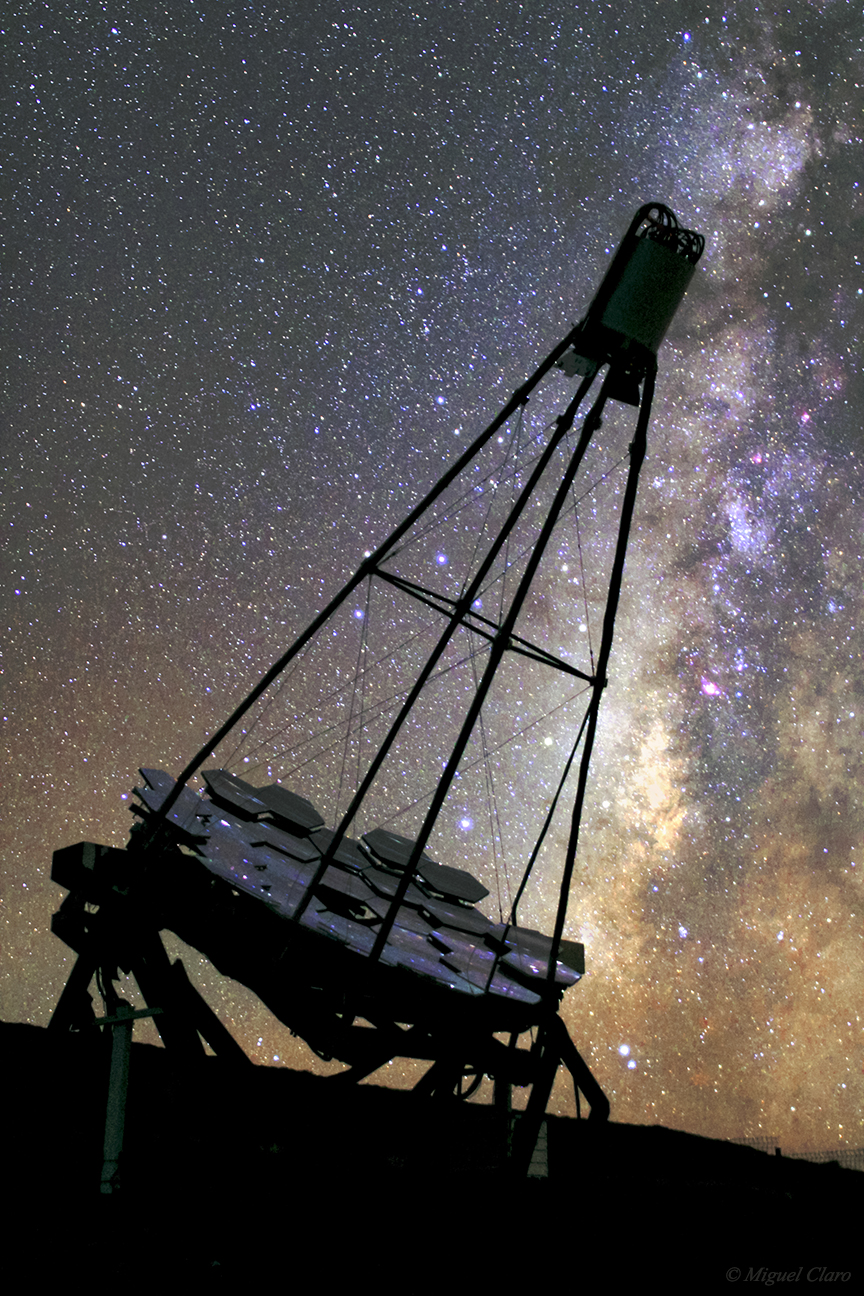
\includegraphics[width=0.5\textwidth]{./logos/FACT.jpg}
  \caption{FACT in Observatiosposition}
  \label{fig:observ}

\end{wrapfigure}
Das FACT (First G-APD Cherenkov Telescope) dient der Überwachung von $\gamma$-Quellen, um bei erhöhter Aktivität, für genauere Observationen größere Telekope zu informieren. Desweiteren erprobt das Telekop die Nutzung von Silizium Photomultiplier (SiMPs) mit welchen es möglich ist, auch an Tagen mit starker diffuser Hintergrundstrahlung Quellen zu observieren. \\

Auf einer höhe von 2200 meter über dem Meeresspiegel befindet sich das Cherenkov Teleskop auf der kanarischen Insel Las Palma. Das Projekt entstand als ein Nachfolgerexperiment des übergebliebenen HEGRA CT3 Telskope, wobei die übergeblieben Spiegel aufbereitet und wiederverwertet werden. (nochmal schöner Formulieren)\\

Die 30 hexongonalen Spiegel bilden eine Gesamtspiegelfläche von \SI{9.51}{\meter\squared} bei einem Blickfeld von \SI{4.5}{\degree}. Die Spiegel sind seid der neuasusrichtung in der Davies-Cotton design ausgerichtet. \cite{??} 
Als erstes Telskope seiner Zeit verwendet FACT SiPMs verwendet anstelle von herkömlichen Photomultiplier Tubes. Halbleiterdetektoren lassen sich mit einer geringerren operation Spannung (< \SI{100}{\volt}) betreiben und sind preiswerter als Photomultiplier, was die Gestaltung des Kameradesigns, als auch die Finanzierung vereinfacht. SiPMs sind aufgrund ihrer hoher Sensitivität dazu in der Laage einzelne Photonen zu detektieren.
Dabei bilden 1440 Kamerapixel das Bild der Kamera, welche jeweils aus einem quadratischen Sensor und einem Plexiglasleiter bestehen. Die einzelne Oberflächen der Hexagonal zulaufenden Plexiglasleiter bilden dabei das Kamerabild.


\section{Wobble Observation Strategy}
